\newpage

\section*{ $^{64}$Zn(n,p)$^{64}$Zn }

Power Level: 100 kW(th) \\
Time at Power: 7200 s \\
Wait Time: 172800 s \\
Total Activity at Removal: 3.54e-01 $\mu Ci$

\begin{table*}[h]
\centering
\begin{tabular}{ |c|c|c|c|c|c| }
 \hline
 Position & Mass $mg$ & Counting Time $s$ & Counting Activity $\mu Ci$ & Expected Area (Counts) \\
 \hline 
 1 & 1.0744186046511628 & 3600 & 4.56e-02 & 4.43e+02\\ 
\hline
 2 & 1.0744186046511628 & 3600 & 7.09e-02 & 6.89e+02\\ 
\hline
 3 & 1.0744186046511628 & 3600 & 6.50e-02 & 6.32e+02\\ 
\hline
 4 & 1.0744186046511628 & 3600 & 2.70e-02 & 2.62e+02\\ 
\hline
\end{tabular}
\end{table*}

\begin{figure}[!ht]
   \centering
   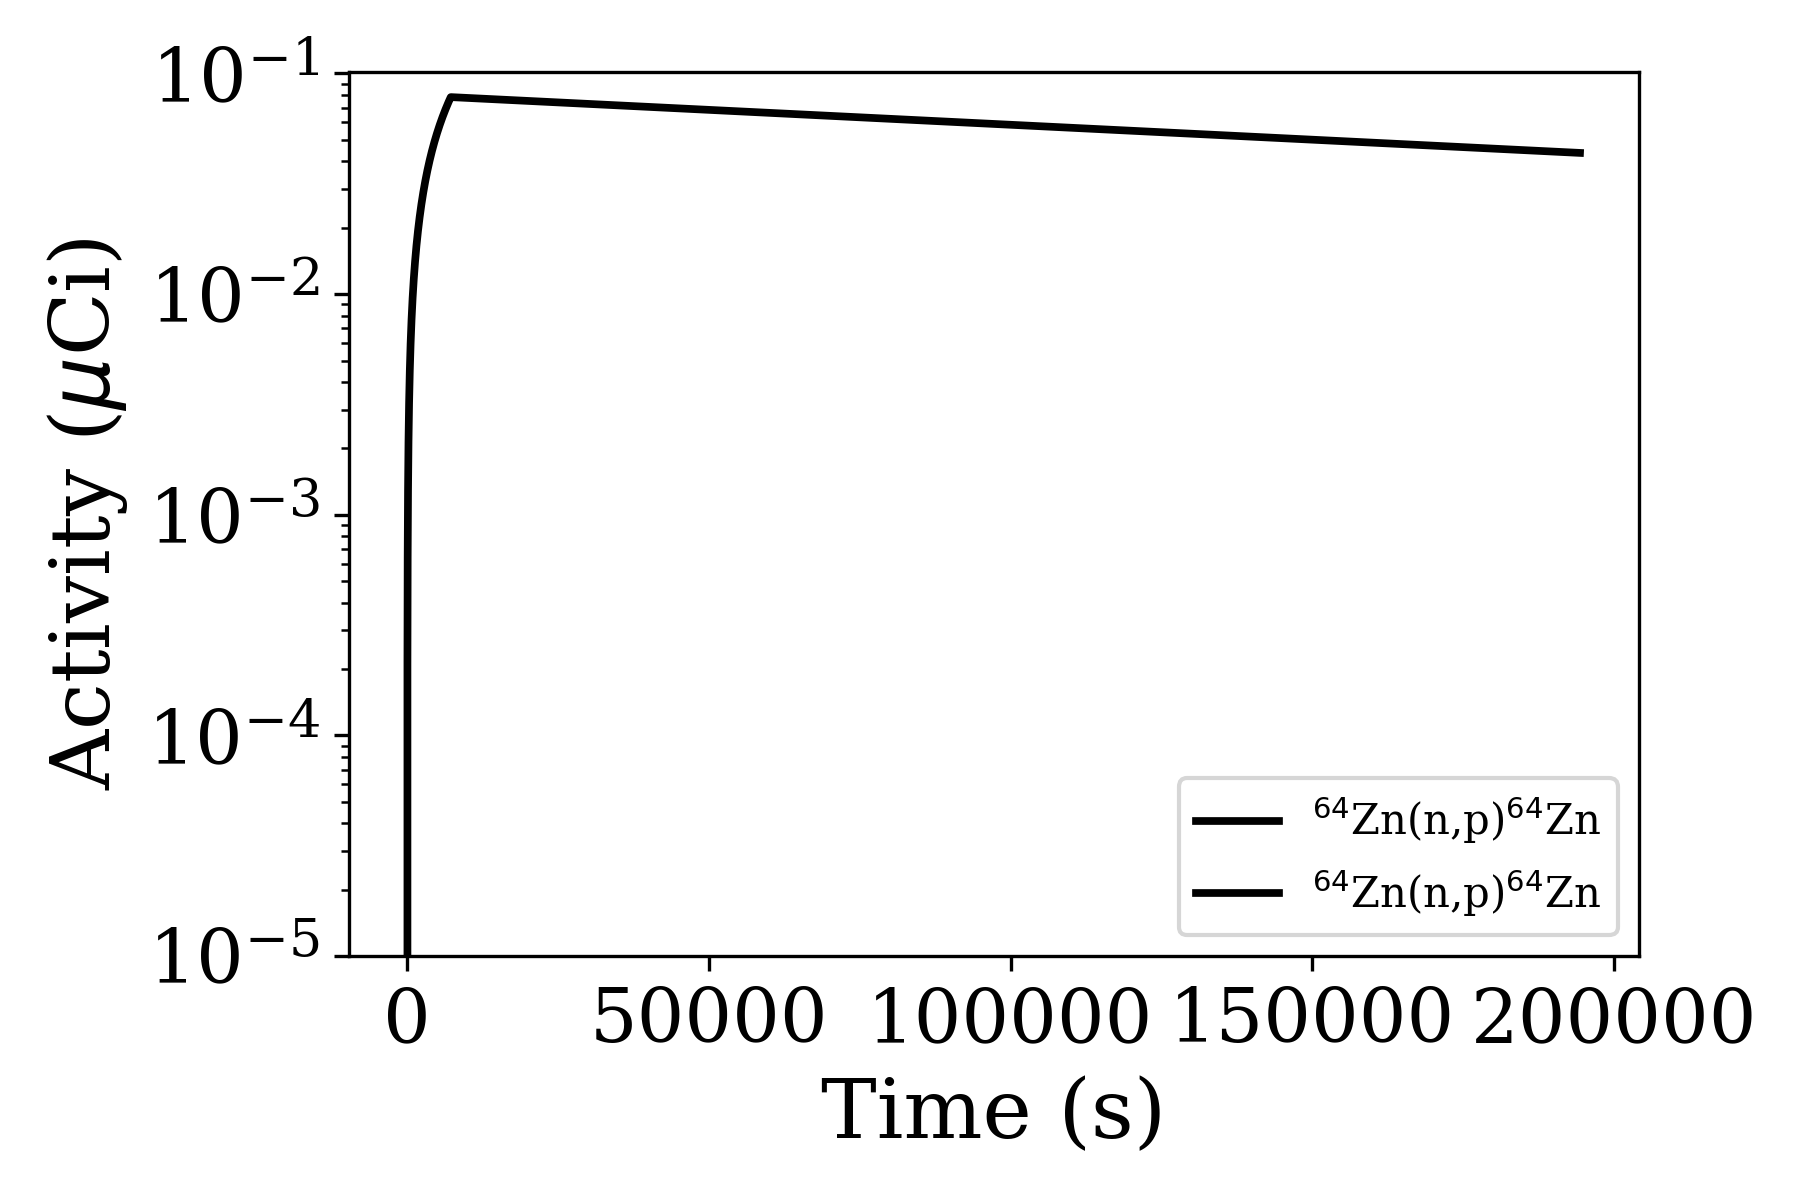
\includegraphics[width=.4\textwidth]{source/plot/Zn-64(n,p)Cu-64_wisconsin1.png} 

\end{figure}

\begin{figure}[!ht]
   \centering
   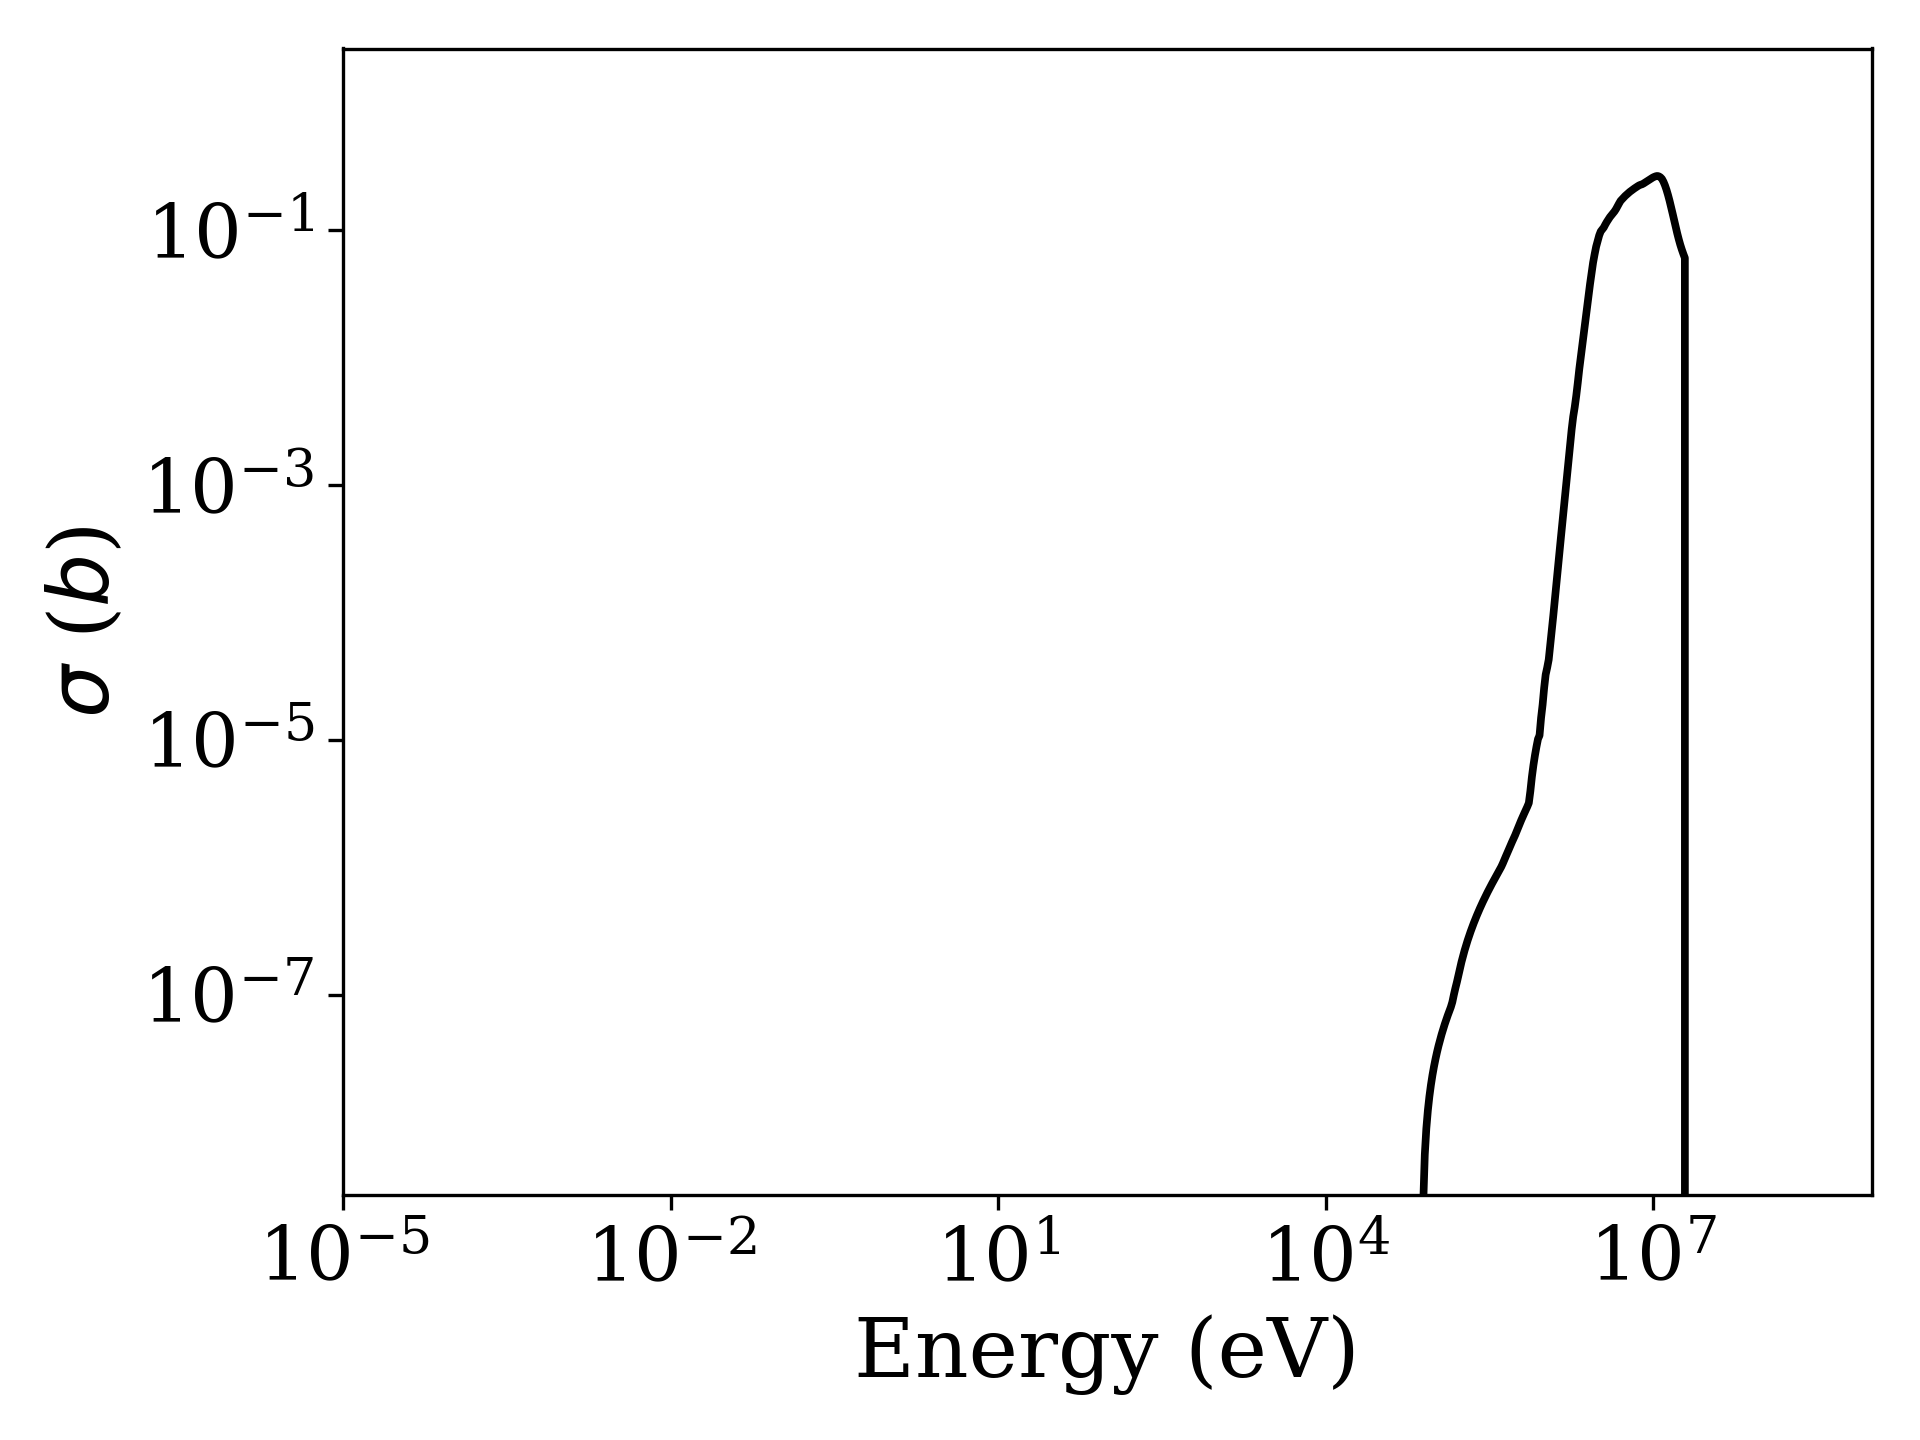
\includegraphics[width=.4\textwidth]{source/plot/Zn-64(n,p)Cu-64.png} 

\end{figure}

\begin{table*}[h]
\centering
\begin{tabular}{ |c|c|c|c|c|c|c| }
 \hline
 Reaction & T$_{1/2}$ & ROI (eV) & Important Gammas (keV) \\
 \hline 
 $^{64}$Zn(n,p)$^{64}$Zn &  2.6 d & 2.47e+06, 8.16e+06 & 1345.77(0.00475),  \\ 
\hline
\end{tabular}
\end{table*}
